% The master copy of this demo dissertation is held on my filespace
% on the cl file serve (/homes/mr/teaching/demodissert/)

% Last updated by MR on 2 August 2001 

\documentclass[12pt,twoside,notitlepage]{report}

\usepackage{pgf}
\usepackage{tikz}
\usetikzlibrary{arrows,automata}
\usepackage[latin1]{inputenc}
\usepackage{verbatim}
\usepackage{tikz}
\usetikzlibrary{arrows,positioning} 
\tikzset{
    %Define standard arrow tip
    >=stealth',
    %Define style for boxes
    punkt/.style={
           rectangle,
           rounded corners,
           draw=black, very thick,
           text width=6.5em,
           minimum height=1em,
           text centered},
    % Define arrow style
    pil/.style={
           ->,
           thick,
           shorten <=2pt,
           shorten >=2pt,}
}

\usepackage{xcolor}
 \usepackage[T1]{fontenc}
 \usepackage{palatino}
 \usepackage{courier}
\usepackage{alltt}
 \usepackage{longtable}
 \DeclareTextSymbol{\QT}{T1}{39}
 \DeclareTextSymbol{\COMMA}{T1}{44}
 \DeclareTextSymbol{\COLON}{T1}{58}
 \DeclareTextSymbol{\SC}{T1}{59}
 \DeclareTextSymbol{\BS}{T1}{92}
 \DeclareTextSymbol{\CI}{T1}{94}
 \DeclareTextSymbol{\TI}{T1}{126}
 \definecolor{navy}{rgb}{0.15, 0.15, 0.45} 
 \definecolor{myblue}{rgb}{0.25, 0.25, 0.645} 
 \definecolor{darkred}{rgb}{0.845, 0.125, 0.125} 
 \definecolor{grey}{rgb}{0.4, 0.4, 0.4} 
 \definecolor{darkgreen}{rgb}{0.125, 0.845, 0.125} 
 \definecolor{leaf}{rgb}{0.1, 0.9, 0.1} 
 
 \newcommand{\mlkeywordA}[1]{\mbox{\color{cyan}{\textbf{\texttt{#1}}}}}
 \newcommand{\mlkeywordB}[1]{\mbox{\color{navy}{\textbf{\texttt{#1}}}}}
 \newcommand{\mlkeyword}[1]{\mbox{\color{red}{#1}}}
 \newcommand{\mloperator}[1]{\mbox{\color{darkgreen}{#1}}}
 \newcommand{\mlmodulename}[1]{\mbox{\color{navy}{#1}}}
 \newcommand{\mlstring}[1]{\mbox{\color{navy}{#1}}}
 \newcommand{\mlcomments}[1]{\mbox{\color{grey}{#1}}}
 \newcommand{\mlcodeline}[2]{\tiny\sl #1 & \begin{minipage}[c]{0.8\linewidth}\begin{alltt}\mbox{#2}\end{alltt}\end{minipage}\\}
 
 \usepackage{a4}
% ---------------------------------------------------------------------


\input{epsf}                            % to allow postscript inclusions
% On thor and CUS read top of file:
%     /opt/TeX/lib/texmf/tex/dvips/epsf.sty
% On CL machines read:
%     /usr/lib/tex/macros/dvips/epsf.tex



\raggedbottom                           % try to avoid widows and orphans
\sloppy
\clubpenalty1000%
\widowpenalty1000%

\addtolength{\oddsidemargin}{6mm}       % adjust margins
\addtolength{\evensidemargin}{-8mm}

\renewcommand{\baselinestretch}{1.1}    % adjust line spacing to make
                                        % more readable

\begin{document}

\bibliographystyle{plain}


%%%%%%%%%%%%%%%%%%%%%%%%%%%%%%%%%%%%%%%%%%%%%%%%%%%%%%%%%%%%%%%%%%%%%%%%
% Title


\pagestyle{empty}

\hfill{\LARGE \bf Dimitar Popov}

\vspace*{60mm}
\begin{center}
\Huge
{\bf Concurrent revisions library for OCaml} \\
\vspace*{5mm}
Part II of the Computer
Science Tripos\\
\vspace*{5mm}
Homerton College \\
\vspace*{5mm}
\today  % today's date
\end{center}

\cleardoublepage

%%%%%%%%%%%%%%%%%%%%%%%%%%%%%%%%%%%%%%%%%%%%%%%%%%%%%%%%%%%%%%%%%%%%%%%%%%%%%%
% Proforma, table of contents and list of figures

\setcounter{page}{1}
\pagenumbering{roman}
\pagestyle{plain}

\chapter*{Proforma}

{\large
\begin{tabular}{ll}
Name:               & \bf Dimitar Popov                     \\
College:            & \bf Homerton College                     \\
Project Title:      & \bf Concurrent revisions library for OCaml \\
Examination:        & \bf Part II of the Computer
Science Tripos, July 2014        \\
Word Count:         & %\bf 1587\footnotemark[1]
\\
Project Originator: & Dr Anil Madhavapeddy                    \\
Supervisor:         & Dr Anil Madhavapeddy                    \\ 
\end{tabular}
}
%\footnotetext[1]{This word count was computed
%by {\tt detex diss.tex | tr -cd '0-9A-Za-z $\tt\backslash$n' | wc -w}
%}
\stepcounter{footnote}


\section*{Original Aims of the Project}

To design and build a library for OCaml that implements the concept of Concurrent revisions. Test the library and implement use cases using the library. Understand the trade offs both between the different paths that can be chosen during the implementation of the library and between the more traditional means of concurrent programming and the concept at hand. Evaluate the differences between the API of the original implementation written in C\# and the more functional one that is natural to OCaml. 


\section*{Work Completed}


\section*{Special Difficulties}


 
\newpage
\section*{Declaration}

I, Dimitar Popov of Homerton College, being a candidate for Part II of the Computer
Science Tripos, hereby declare
that this dissertation and the work described in it are my own work,
unaided except as may be specified below, and that the dissertation
does not contain material that has already been used to any substantial
extent for a comparable purpose.

\bigskip
\leftline{Signed }

\medskip
\leftline{Date }

\cleardoublepage

\tableofcontents

\listoffigures

\newpage
\section*{Acknowledgements}


%%%%%%%%%%%%%%%%%%%%%%%%%%%%%%%%%%%%%%%%%%%%%%%%%%%%%%%%%%%%%%%%%%%%%%%
% now for the chapters

\cleardoublepage        % just to make sure before the page numbering
                        % is changed

\setcounter{page}{1}
\pagenumbering{arabic}
\pagestyle{headings}

\chapter{Introduction}

\section{Overview of the project}
The biggest challenge when using parallel programming is typically how to keep track of the side effects of computations that are executed in parallel. Traditional method for dealing with this issue often limit concurrency, do not provide sufficient determinism and are error prone. Ideally, we would like a concept where all conflict between parallel tasks are resolved deterministically with as less as possible effort from the programmer. 

One concept that satisfies these requirements is that of Concurrent Revisions, initially proposed at OOPSLA'10 [1]. The aim of this projec is to implement this concept in the functional language OCaml and evaluate its performance and usability. The domain of functional languages was chosen because of their inherited determinism which makes using parallelism less complex and provides a facility for tracking side effects. I have designed and implemented a library that incorporates the ideas of Concurrent Revisions and ensured its correctness with a number of unit tests. Together with some small example code, two use cases were produced using the library - a logging system and a chat service. They were used to evaluate the performance and usability of the implementation and the whole concept in the world of OCaml. The conclusion was that [add when actually have a conclusion].  

\section{Overview of Concurrent revisions}

The idea of Concurrent revisions as initially proposed highlights three main design choices:
\begin{itemize}
\item {\bfseries Declarative data sharing} - the user declares what data is to be shared between parallel tasks by the use of isolation types.

\item {\bfseries Automatic isolation} - each task has its own private stable copy of the data that is created at the time of the fork.

\item {\bfseries Deterministic conflict resolution} - the user also specifies a merge function that is used to resolve write-write conflicts at that might arise when joining parallel tasks. Given that this function is deterministic, the conflict resolution is also deterministic.

\end{itemize}

In this framework the unit of concurrency are asynchronous tasks called revisions. They allow the typical functionality for asynchronous tasks - the user can create, fork and join them. This removes the complexity of synchronization out of the tasks themselves and gathers in into a single place - the merge function. 

\section{Motivation}

\subsection{Overview of other approaches to concurrency}
 
Concurrency is essential and vital in multi core architectures and in distributed systems. Traditional approaches rely on synchronizing parallel tasks by locks, event driven formalisms or similar. This makes conflicts very expensive if determinism is needed. Moreover, these methods are often error prone and extremely hard to debug.

Standard locking schemes are sometimes a good approach to ensure consistency of data shared between multiple parallel tasks. However locking limits concurrency since task are blocked until it is safe to continue. Significant effort is required from the programmer to reason about all possible interleaves of task execution. Identifying the scope of critical sections becomes tricky as it could either limit concurrency or insufficient isolation. This approach is highly error prone and extremely difficult to maintain.

Instead of locking one can use event-driven systems, where tasks execution is triggered by event from other tasks.  This results in inverted control structure of the program. The programmer's control flow becomes inverted and results into convoluted control logic. In such a system, often the actual tasks have to be very fine grained in order to maximize performance which complicates the logic and makes it difficult to maintain.

Another approach is instead of trying to avoid conflicts to try to resolve them. This is in the core of transactional systems in which each tasks takes a copy of the shared data and conflicts are resolved at the time of the join. However conflicts are resolved non-deterministically which complicates reasoning about the execution. Another criticism of transactional systems is that they ensure serializability, which is not necessary for all use cases and limits concurrency[4].   

In the concept of concurrent revisions the guarantee of parallel executions being equivalent to some sequential schedule is relaxed. Instead, given the right abstractions, the programmer can reason about the execution directly. 

This approach is data centric in a sense that it takes the complexity of synchronization out of the tasks and adds it to the data declarations.  

\subsection{The contribution of Concurrent revisions}

Much like transactional systems, Concurrent revisions use replication to ensure isolation. Because of that roll-back of aborted revisions comes for free. The guarantee of parallel executions being equivalent to some sequential schedule is relaxed. This increases parallelism and leaves to the programmer only to things to worry about - what has to be shared and how conflicts have to be resolved, concentrating any possible bugs in a limited region. With Concurrent revisions, given the right abstractions, the programmer can reason about the execution directly making the design of a concurrent system much natural.

This approach is data centric in a sense that it takes the complexity of synchronization in terms of programmer effort out of the tasks and adds it to the data declarations. The runtime complexity of synchronization is shifted from blocking or checking that the schedule of tasks was legal into the join of tasks where conflicts are resolved by a deterministic computation.   

\subsection{Applicable areas}
Every system that is subject to a lot of conflicts typically has to limit the parallelism of its execution in order to ensure consistency and avoid conflicts. Concurrent revisions take the different approach of resolving conflicts instead of avoiding them by scheduling. This makes them suitable for problems where there are a lot of write-write conflicts which should be resolved deterministically and performance can be increased greatly by more parallelism. Some examples of applications that could benefit from concurrent revisions are: 

\begin{itemize}


\item
{\bfseries Bank transactional systems} - Such systems have a lot of constraints on invariants that form write- and read-skews. We will see later how this can nicely be resolved if using concurrent revisions[reference].

\item
{\bfseries Games} - They are a natural example when high parallelism is crucial for adequate performance. However, the fact that there are a lot of conflicts-user input, graphics rendering, simulating physics and logic, write-back to disk, makes getting their parallelization right tricky. Now what if we execute each of these tasks in separate revision and then join them as appropriate. There is one more concern of course - we have to be able to resolve conflicts. Luckily in order to do so, we simple have to define the merge function, which bundles all the complexity of dealing with conflicts into a single place, making it much more maintainable. Getting the merge function right is crucial, as we do not want our player to dash in a wall that was not displayed on the screen yet.

\item
{\bfseries Logging \& Chat systems} - The usage of functional languages for large commercial systems is increasing in large distributed systems such as logging and chat systems. One example of that is the Facebook chat, which is written in Erlang. Such systems are often large and distributed and have a lot of conflicts, timing and consistency are vital and it more or less requires deterministic behaviour. This matches the list of requirements for suitability of concurrent revisions and we will see later that it is indeed convenient to write a chat server using them.

\end{itemize}

\subsection{Why OCaml?}

OCaml is functional programming language that is getting increasingly more popular both in academia and in the industry. The increasing amount of libraries for OCaml makes it an excellent choice for a variety of use cases. 

As a functional language provides a natural means of tracking executions by the use of the type checker and the convenience of using immutable data types. Replication of complex immutable data structures in OCaml are very cheap, since no actual replication is done, but rather upon updates the structure of the old value is heavily reused, which makes updates cost only constant space.

These features of OCaml makes it a very efficient environment for implementation of Concurrent Revisions.

One down-side of OCaml is its limited parallelism. The run-time system is single threaded which means that there is only one parallel task ever in execution. There is no guarantee on the scheduling and interleaving of tasks which makes it non-trivial to writer parallel software in OCaml. Due to this fact, there is no performance improvement expected when using revisions. The key benefits of using revisions are better responsiveness at the cost of little overhead and decreased amount of effort required by the programmer.   

\section{Quick overview of OCaml, the Core and Async libraries}
OCaml is a garbage-collected functional language that also has object-oriented features.
This section gives a brief overview of the features of OCaml used in the project.

\subsection{Basic Types}
As every functional language OCaml has a strong-type system that is incredibly useful in spotting bugs at compile type. The most heavily used types in OCaml are immutable. Here is an example of these:

%let x = 1

%let x = 2 in
%  print_int(x)

%let z = ("Hello", 1, 3.14)

%let l = [1,2,3] 

{\scriptsize\noindent\begin{longtable}{r|l}
\mlcodeline{1}{\mlkeywordA{let}~x~\mlkeyword{=}~1
}
\mlcodeline{2}{
}
\mlcodeline{3}{\mlkeywordA{let}~x~\mlkeyword{=}~2~\mlkeywordA{in}
}
\mlcodeline{4}{~~print\_{}int(x)
}
\mlcodeline{5}{
}
\mlcodeline{6}{\mlkeywordA{let}~z~\mlkeyword{=}~(\mlstring{"Hello"}\mloperator{\mbox{,}}~1\mloperator{\mbox{,}}~3.14)
}
\mlcodeline{7}{
}
\mlcodeline{8}{\mlkeywordA{let}~l~\mlkeyword{=}~\mloperator{[}1\mloperator{\mbox{,}}2\mloperator{\mbox{,}}3\mloperator{]}
}

\end{longtable}
}

On line 1 the user declares the variable {\tt x} and assigns it the value of 1.  This value is immutable and cannot be assigned to again.  It can only be shadowed by another variable of the same name. The type checker resolves the type of {\tt x} as {\tt int}. The {\tt let} binding specifies the scope of the declaration. In this case the variable {\tt x} has a scope form line 1 to the end of the program. The {\tt let ... in} binding allows us to declare a scope for the variable. On line 3 you can see that {\tt x} is shadowed by another variable with scope until the end of line 4. There are also tuple data types, an example of which you can see on line 6. Here {\tt z} contains 3 values of different types. The type of z is {\tt string*int*float}. On line 8 we can see an example of a list. Lists in OCaml are implemented a single-linked lists and a pointer to the head of the lists. Which makes most access and update operations on list linear in time. Lists are also immutable. Updates reuse the structure of the old list and only replace the updated values, making them very space efficient.

Another important set of types are the functional types. Here is an example:

%let add a b = a + b

%let rec factorial n = n * (factorial (n-1))  

{\scriptsize\noindent\begin{longtable}{r|l}
\mlcodeline{1}{\mlkeywordA{let}~add~a~b~\mlkeyword{=}~a~\mloperator{+}~b
}
\mlcodeline{2}{
}
\mlcodeline{3}{\mlkeywordA{let~rec}~factorial~n~\mlkeyword{=}~n~\mloperator{*}~(factorial~(n-1))~~}
\end{longtable}
} 

The function {\tt add} is of type {\tt int -> int -> int}, takes two integer arguments and returns one integer result. The function factorial is a recursive function. Recursive is very important in functional languages as they are centered on the data structures, which are typically hierarchical, making it natural to operate on them in a recursive manner. OCaml can have functions from every OCaml type to every OCaml type as well as polymorphic functions.

Other basic structures include variants and records:

%type point2d = { x : float; y : float }

%type option = None
%             |Some of 'a 

{\scriptsize\noindent\begin{longtable}{r|l}
\mlcodeline{1}{\mlkeyword{type}~point~\mlkeyword{=}~\mloperator{\{}~x~\mloperator{\mbox{\COLON}}~float\mloperator{\mbox{\SC}}~y~\mloperator{\mbox{\COLON}}~float~\mloperator{\}}
}
\mlcodeline{2}{
}
\mlcodeline{3}{\mlkeyword{type}~option~\mlkeyword{=}~None
}
\mlcodeline{4}{~~~~~~~~~~~~~\mloperator{|}Some~\mlkeyword{of}~'a
}
\end{longtable}
}
Each variable of type {\tt point} has two fields {\tt y} and {\tt x} both of type integer. This is called record type. The type {\tt option} is a variant type. A variable of type {\tt option} can either be equal to {\tt None} or {\tt Some(x)}. Notice the type {\tt 'a} this specifies a polymorphic type meaning {\tt x} can be of any type.

OCaml also has imperative features:

%let x = ref 1

%x := !x + 2 

{\scriptsize\noindent\begin{longtable}{r|l}
\mlcodeline{1}{\mlkeywordA{let}~x~\mlkeyword{=}~ref~1
}
\mlcodeline{2}{
}
\mlcodeline{3}{x~\mloperator{\mbox{\COLON}{}=}~\mloperator{\mbox{}\hspace{0pt}{!}\hspace{0pt}}x~\mloperator{+}~2~
}
\end{longtable}
}

Here {\tt x} is declared as a {\tt int ref} and is a reference to a particular place in memory. The value of {\tt x} itself cannot be changed. What can be changes of the value of the place where it points to. On line 3 {\tt x} is updated by assigning to it the sum of the dereferenced value of {\tt x} and 2.  


\subsection{Complex data structures from the Core library}
The Core library is a wrapper around the standard OCaml library that provides additional features. It this project I used the map and set data structures that are implemented as AVL trees. AVL tree is a self-balanced binary search tree that guarantees a logarithmic complexity for insertions, deletions and updates due to its balanced structure. Both these data structures are immutable, allowing them to share great proportion of their internal structure. This makes replication cheap both in terms of space and time. 

\subsection{Module system}
The module system is a key feature of OCaml. It can be used to package together related definitions. For example one can package a particular data type together with the associated operations over that type and abstract away the actual implementation of that type. Here is an example of a simple module:

%module Balance : sig
%  type t
%  val add: t -> t -> t
%  val of_int: int -> t
%end = struct
%  type t = int
%  let add a b = a + b
%  let of_int x = x
%end


{\scriptsize\noindent\begin{longtable}{r|l}
\mlcodeline{1}{\mlkeywordA{module}~Balance~\mloperator{\mbox{\COLON}}~\mlkeyword{sig}
}
\mlcodeline{2}{~~\mlkeyword{type}~t
}
\mlcodeline{3}{~~\mlkeyword{val}~add\mloperator{\mbox{\COLON}}~t~\mlkeyword{->}~t~\mlkeyword{->}~t
}
\mlcodeline{4}{~~\mlkeyword{val}~of\_{}int\mloperator{\mbox{\COLON}}~int~\mlkeyword{->}~t
}
\mlcodeline{5}{\mlkeyword{end}~\mlkeyword{=}~\mlkeyword{struct}
}
\mlcodeline{6}{~~\mlkeyword{type}~t~\mlkeyword{=}~int
}
\mlcodeline{7}{~~\mlkeywordA{let}~add~a~b~\mlkeyword{=}~a~\mloperator{+}~b
}
\mlcodeline{8}{~~\mlkeywordA{let}~of\_{}int~x~\mlkeyword{=}~x
}
\mlcodeline{9}{\mlkeyword{end}}
\end{longtable}
}
Here from line 1 to 4 is declared the signature to the module {\tt Balance}. This is the interface available when using the module. The actual implementation of the module is from line 5 to 9. It has to comply to the signature of the module.

A valuable feature when dealing with modules are the functors. Here is an example of using a functor:

%module IntSet = 
%   Set.Make(struct
%             type t = int
%             let compare x y = Int.compare x y
%            end)

{\scriptsize\noindent\begin{longtable}{r|l}
\mlcodeline{1}{\mlkeywordA{module}~IntSet~\mlkeyword{=}~
}
\mlcodeline{2}{~~~\mlmodulename{Set}\mbox{}\mloperator{.}Make(\mlkeyword{struct}
}
\mlcodeline{3}{~~~~~~~~~~~~~\mlkeyword{type}~t~\mlkeyword{=}~int
}
\mlcodeline{4}{~~~~~~~~~~~~~\mlkeywordA{let}~compare~x~y~\mlkeyword{=}~\mlmodulename{Int}\mbox{}\mloperator{.}compare~x~y
}
\mlcodeline{5}{~~~~~~~~~~~~\mlkeyword{end})}
\end{longtable}
}

Here I am using the build-in in Core functor {\tt Set.Make} to create an integer set. The functor expect a module with a signature that requires the type of the set elements, i.e {\tt t}, and a comparison function between elements. Notice the use of the build-in function from the module {\tt Int} on line 4.

\subsection{The Async concurrency library}
The Async library was used as the exclusive source of parallelism throughout the project. Async is a monadic concurrency library. It is build around the idea of deferred computations that are scheduled non-deterministically. It has a global lock that ensures only one computation will be in execution at any given time. Each computation is executed atomically which guarantees two computations will never overlap. The most common pattern for programming with Async is to schedule new computations to be executed over the outputs of a previous computation once they are determined. This results in a guarantee for a sequence of actions to be performed in a particular order. Example taken from [3]:

%Reader.file_contents filename
%   >>| fun text ->
%   List.length (String.split text ~on:'\n')  

{\scriptsize\noindent\begin{longtable}{r|l}
\mlcodeline{1}{\mlmodulename{Reader}\mbox{}\mloperator{.}file\_{}contents~filename
}
\mlcodeline{2}{~~~\mloperator{>\mbox{}>\mbox{}|}~\mlkeyword{fun}~text~\mlkeyword{->}
}
\mlcodeline{3}{~~~\mlmodulename{List}\mbox{}\mloperator{.}length~(\mlmodulename{String}\mbox{}\mloperator{.}split~text~\mloperator{\TI}on\mloperator{\mbox{\COLON}}'\mloperator{\BS}n')}
\end{longtable}
}

Here on line 1 we schedule a deferred computation that reads the context of a file. On line 2 we bind it to a function that will be scheduled after the output of the read operation is determined, upon which it computes the number of lines in the file.

This pattern can be used to overcome the problem of the blocking nature of reading and writing to streams, when they are respectively empty or full.

\section{Deeper look into the concept}
\subsection{Data structures \& Runtime behaviour }

The main data structure in the concept are the revisions. They can be seen as a stable context for each asynchronous task as they are isolated of each other. The isolation types encapsulate the structure of the data to be shared. 

Let's look at a simple example:

%IntRevision example
%IntIsolated = isolate(int)
%IntRevision = Revision.make(IntIsolated, 
%                  fun head parent current -> head + current - parent)
%(account, revision) = IntRevision.create 0
  
%let rev1 = revision.fork(fun r -> account = account + 5)
%let rev2 = revision.fork(fun r -> account = account + 10)
  
%assert(account in revision = 0)
%assert(account in rev1 = 5)
%assert(account in rev2 = 10)
  
%let rev_join1 = join rev rev1
%let rev join2 = join rev_join1 rev2
  
%assert(account in rev_join1 = 5)
%assert(account in rev_join2 = 15) 
{\scriptsize\noindent\begin{longtable}{r|l}
\mlcodeline{1}{IntIsolated~\mlkeyword{=}~isolate(int)
}
\mlcodeline{2}{IntRevision~\mlkeyword{=}~\mlmodulename{Revision}\mbox{}\mloperator{.}make(IntIsolated\mloperator{\mbox{,}}~
}
\mlcodeline{3}{~~~~~~~~~~~~~~~~~~\mlkeyword{fun}~head~parent~current~\mlkeyword{->}~head~\mloperator{+}~current~\mloperator{-}~parent)
}
\mlcodeline{4}{(account\mloperator{\mbox{,}}~revision)~\mlkeyword{=}~\mlmodulename{IntRevision}\mbox{}\mloperator{.}create~0
}
\mlcodeline{5}{~~
}
\mlcodeline{6}{\mlkeywordA{let}~rev1~\mlkeyword{=}~revision\mloperator{.}fork(\mlkeyword{fun}~r~\mlkeyword{->}~account~\mlkeyword{=}~account~\mloperator{+}~5)
}
\mlcodeline{7}{\mlkeywordA{let}~rev2~\mlkeyword{=}~revision\mloperator{.}fork(\mlkeyword{fun}~r~\mlkeyword{->}~account~\mlkeyword{=}~account~\mloperator{+}~10)
}
\mlcodeline{8}{~~
}
\mlcodeline{9}{\mlkeyword{assert}(account~\mlkeywordA{in}~revision~\mlkeyword{=}~0)
}
\mlcodeline{10}{\mlkeyword{assert}(account~\mlkeywordA{in}~rev1~\mlkeyword{=}~5)
}
\mlcodeline{11}{\mlkeyword{assert}(account~\mlkeywordA{in}~rev2~\mlkeyword{=}~10)
}
\mlcodeline{12}{~~
}
\mlcodeline{13}{\mlkeywordA{let}~rev\_{}join1~\mlkeyword{=}~join~rev~rev1
}
\mlcodeline{14}{\mlkeywordA{let}~rev~join2~\mlkeyword{=}~join~rev\_{}join1~rev2
}
\mlcodeline{15}{~~
}
\mlcodeline{16}{\mlkeyword{assert}(account~\mlkeywordA{in}~rev\_{}join1~\mlkeyword{=}~5)
}
\mlcodeline{17}{\mlkeyword{assert}(account~\mlkeywordA{in}~rev\_{}join2~\mlkeyword{=}~15)~}
\end{longtable}
}
Example 1.\\



 
On line 1 the programmer creates a isolation type that isolates the primitive type integer. Then on line 2 and 3, he creates a {\tt IntRevision} module by specifying the isolated type and the merge function. This function takes three arguments - the value of the isolated in the revision we are joining to, the value at the time of the fork and the current value in the joinee. Then he creates a revision specifying initial value for the isolated to be 0. This returns a tuple with type {\tt IntIsolated.t * IntRevision.t}. The user than can use {\tt account} to access its value in different revisions. 

One line 6 and 7 we fork two new revisions that would credit the account with 5 and 10 pounds respectively. At this point {\tt account} has different value in each of the three revisions.

Then we join the two new revisions one by one to our main initial revision (line 13 \& 14). Luckily due to how we specified the merge function and the deterministic nature of the approach, we account has the right amount at the end - 15 pounds.

If we have used a more traditional approach, we would have had to lock the whole system each time we access the value of the account, while now we simply synchronize it when we join the tasks. 

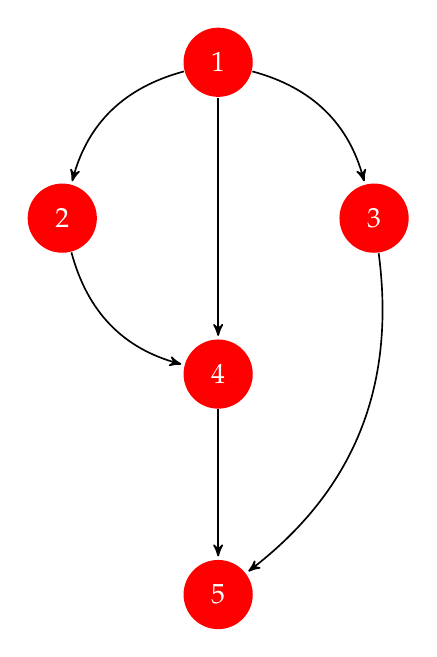
\begin{tikzpicture}[->,>=stealth',shorten >=1pt,auto,node distance=2.8cm,
                    semithick]
  \tikzstyle{every state}=[fill=red,draw=none,text=white]

  \node[state] (A)                    {1};              
  \node[state]         (B) [below right of=A] {3};
  \node[state]         (C) [below left  of=A] {2};
  \node[state]         (D) [below left of=B] {4};
  \node[state]         (E) [below of=D]       {5};



        
  \path (A) edge [bend left]  node {} (B)
            edge [bend right]   node {} (C)
            edge               node{}       (D)
        (C) edge [bend right] node{} (D) 
        (D) edge node{} (E)
        (B) edge [bend left] node{} (E)   
        ;      
\end{tikzpicture}
 
Fig.1: Revision diagram of Example 1. In the following diagram the nodes are the revisions. Outgoing arrows represent forks and  joins are represented by incoming arrows, which are always two, one straight for the revision we are joining to and one bend for the joinee. In the diagram nodes correspond to revisions as follows: 1 - {\tt revision } 2 - {\tt rev1 } 3 - {\tt rev2 } 4 - {\tt join\_rev1 } 5 - {\tt join\_rev2}  

\subsection{Illegal revision diagrams}
Not all possible joins are legal as some of them might invalidate the assumptions about the flow of revisions. Consider these examples of illegal diagrams:

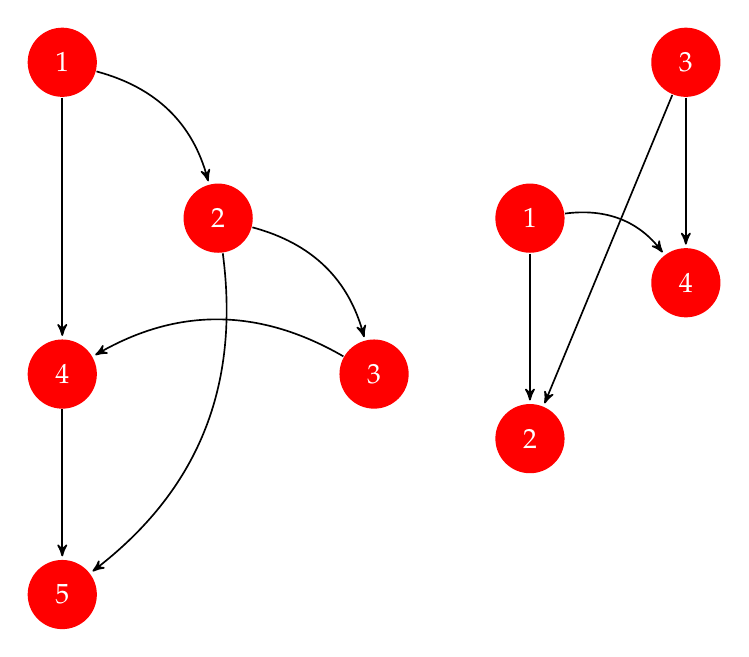
\begin{tikzpicture}[->,>=stealth',shorten >=1pt,auto,node distance=2.8cm,
                    semithick]
  \tikzstyle{every state}=[fill=red,draw=none,text=white]

  \node[state]         (A)                    {1};              
  \node[state]         (B) [below right of=A] {2};
  \node[state]         (C) [below right  of=B] {3};
  \node[state]         (D) [below left of=B] {4};
  \node[state]         (E) [below of=D]       {5};

  \node[state]         (F) [above right of=C]         {1};
  \node[state]        (G) [below of=F]         {2};
  \node[state]         (H) [above right of=F]         {3};
  \node[state]         (I) [below of=H]        {4};
        
  \path (A) edge [bend left]  node {} (B)
            edge               node{}       (D)
        (C) edge [bend right] node{} (D) 
        (D) edge node{} (E)
        (B) edge [bend left] node{} (C)
            edge [bend left] node{} (E)
            
        (F) edge node{} (G)
            edge [bend left] node{} (I)
        (H) edge node{} (I)
            edge  node{} (G)           
        ;      
\end{tikzpicture}
\\Fig.2: Illegal revision diagrams.
\vspace{10pt}

In Fig.2 we can see two illegal revision diagrams. In the first one, we join revision 3 to revision 1 before we have joined revision 2 which is the parent revision of 3. This means that the result in revision 5 might not be what we would expect since it is unknown how much of the work done in the fork for revision was done before forking revision 3. When we join 2, some of the changes occurring (which might have subsequently been modified) in 2 are already joined when 3 was joined. Since the merge function cannot account for such an interleaving as it is chosen by the programmer arbitrarily, such a revision diagram is not valid. One can imagine a more complex concept that this is accounted for at the time of the join. However this would require significantly more programming effort when designing the merge function. This would result in more difficult to reason about concept, prone to programming error, without adding extra functionality, because the legal revision diagrams area already expressive enough. 

In the second example, we are interleaving two separate flows of revisions and there is no way to ensure that they isolate a similar state. This is completely meaningless, since they could isolate different variables and represent unrelated states.

\subsection{Concurrent revisions in the world of OCaml}
The OCaml implementation of Concurrent Revisions is presented in chapter 3. One of its advantages over the C\# implementation is that it is purely functional and the type checker catches some of the typical mistakes that can be made - trying to access an isolated of a wrong type or join revisions of different types. What it does not do however is check for all types of illegal revision diagrams, instead an exception is raised whenever a illegal join is performed. This is far from ideal and statically type-checking joins for compatibility could be implemented as a future extension.

The API that the implementation exposes to the user is intuitive and resembles the typical OCaml approach for APIs for external libraries. Here is a simple example of its usage:
\begin{comment}
module IntRevision = Make(struct
    type t = int
    let merge head parent current = head + current - parent
  end)

let () =
  let r = IntRevision.init () in
  let res1 = IntRevision.create r 0 in
  let revision = IntRevision.get_revision res1 
   and account = IntRevision.get_isolated res1 in
     Deferred.both 
      (IntRevision.fork revision 
        (fun r -> return (IntRevision.write r account ((IntRevision.read r account) + 5)))
      (IntRevision.fork revision 
        (fun r -> return (IntRevision.write r account ((IntRevision.read r account) + 10)))
     >>|(fun (rev1, rev2 ->
        let join_rev1 = IntRevision.join revision rev1 in
        let join_rev2 = Intrevision.join join_rev1 rev2 in
          assert(IntRevision.read join_rev2 = 15)  
\end{comment}


{\scriptsize\noindent\begin{longtable}{r|l}
\mlcodeline{1}{\mlkeywordA{module}~IntRevision~\mlkeyword{=}~Make(\mlkeyword{struct}
}
\mlcodeline{2}{~~~~\mlkeyword{type}~t~\mlkeyword{=}~int
}
\mlcodeline{3}{~~~~\mlkeywordA{let}~merge~head~parent~current~\mlkeyword{=}~head~\mloperator{+}~current~\mloperator{-}~parent
}
\mlcodeline{4}{~~\mlkeyword{end})
}
\mlcodeline{5}{
}
\mlcodeline{6}{\mlkeywordA{let}~()~\mlkeyword{=}
}
\mlcodeline{7}{~~\mlkeywordA{let}~r~\mlkeyword{=}~\mlmodulename{IntRevision}\mbox{}\mloperator{.}init~()~\mlkeywordA{in}
}
\mlcodeline{8}{~~\mlkeywordA{let}~res1~\mlkeyword{=}~\mlmodulename{IntRevision}\mbox{}\mloperator{.}create~r~0~\mlkeywordA{in}
}
\mlcodeline{9}{~~\mlkeywordA{let}~revision~\mlkeyword{=}~\mlmodulename{IntRevision}\mbox{}\mloperator{.}get\_{}revision~res1~
}
\mlcodeline{10}{~~~\mlkeywordA{and}~account~\mlkeyword{=}~\mlmodulename{IntRevision}\mbox{}\mloperator{.}get\_{}isolated~res1~\mlkeywordA{in}
}
\mlcodeline{11}{~~~~~\mlmodulename{Deferred}\mbox{}\mloperator{.}both~
}
\mlcodeline{12}{~~~~~~(\mlmodulename{IntRevision}\mbox{}\mloperator{.}fork~revision~
}
\mlcodeline{13}{~~~~~~~~(\mlkeyword{fun}~r~\mlkeyword{->}~return~(\mlmodulename{IntRevision}\mbox{}\mloperator{.}write~r~account~((\mlmodulename{IntRevision}\mbox{}\mloperator{.}read~r~account)~\mloperator{+}~5)))
}
\mlcodeline{14}{~~~~~~(\mlmodulename{IntRevision}\mbox{}\mloperator{.}fork~revision~
}
\mlcodeline{15}{~~~~~~~~(\mlkeyword{fun}~r~\mlkeyword{->}~return~(\mlmodulename{IntRevision}\mbox{}\mloperator{.}write~r~account~((\mlmodulename{IntRevision}\mbox{}\mloperator{.}read~r~account)~\mloperator{+}~10)))
}
\mlcodeline{16}{~~~~~\mloperator{>\mbox{}>\mbox{}|}(\mlkeyword{fun}~(rev1\mloperator{\mbox{,}}~rev2~\mlkeyword{->}
}
\mlcodeline{17}{~~~~~~~~\mlkeywordA{let}~join\_{}rev1~\mlkeyword{=}~\mlmodulename{IntRevision}\mbox{}\mloperator{.}join~revision~rev1~\mlkeywordA{in}
}
\mlcodeline{18}{~~~~~~~~\mlkeywordA{let}~join\_{}rev2~\mlkeyword{=}~\mlmodulename{Intrevision}\mbox{}\mloperator{.}join~join\_{}rev1~rev2~\mlkeywordA{in}
}
\mlcodeline{19}{~~~~~~~~~~\mlkeyword{assert}(\mlmodulename{IntRevision}\mbox{}\mloperator{.}read~join\_{}rev2~\mlkeyword{=}~15)~~}
\end{longtable}
}

Example 2.\\

In Example 2 we can see the actual implementation of the pseudo code in Example 1. From line 1 to 4 we create the {\tt IntRevision} module using a simple anonymous module specifying the type of the isolated data and the merge function. Then on line 7 we initialize an empty revision and on 8 we add a new isolated to the initial revision to create a new one. We then fork the two asynchronous account credits (line 11 to 14) and later join them. 

This API is not as straight forward as the one in the C\# implementations for couple of reasons. Firstly since it is purely functional, revisions are immutable which requires to create a new revision at each join. Secondly, we need to explicitly create new isolated variables. In the C\# implementation the user simply declares which variables have to be isolated and then uses then accesses them as any regular variables, without explicit read and write operators to which he also has to specify the revision context. The solution in the project implementation is a bit less convenient, it uses special read and write methods, to which the context has to be explicitly stated. However, it makes it much clearer what is actually isolated and when it is accessed and in what context, resulting in a more comprehensive code.  Another drawback of my implementation is that it does not allow having isolated from different types in a single revision, a trivial workaround for which is to use tuples or another complex data structure. I considered using a universal OCaml type as an alternative. Universal types in OCaml however can be implemented only using exceptions which are highly inefficient. 




\cleardoublepage



\chapter{Preparation}
\section{The author in the world of Concurrency}
As part of my degree I have gained broad knowledge of the problems that arise from Concurrency and the typical approaches for solving them. The Concurrent and Distributed Systems course gave me most insight into why and how Concurrent revisions can be used for parallel programming. After reading the original paper, the concept naturally fit in and expanded the mental model I have created about the issues and solutions in the world of Concurrency.  

\section{Familiarizing with the OCaml programming language}
Prior to starting the project, I had almost no experience with the OCaml programming language. For that reason I dedicated the first part of my project to making myself familiar with it. I used the Real World OCaml book [3] to guide me through the concepts and patterns for the language. I was able to quickly transfer and expand my skills in ML into OCaml without much difficulty.

\section{The Core and Async libraries}
I made extensive use of the Core and Async libraries for OCaml. The latter was used in the core of the implementation and the use cases. The Revision module conforms to the pattern of deferred computations in the Async library. This naturally happened in the development process, since the the core concepts in the Async library and those of the project complement each other. The revision and isolated data types are completely isolated, making it trivial to implement them as deferred data types and the forks and the joins as deferred computations.  

\section{Back-up and revision control}
For revision control I used git, with which I had a lot of experience. I used GitHub for back-up of the code. To ensure myself in event of hardware failure of my personal laptop, I kept my whole development environment inside a VM. The VM was backed up on an external hard drive so in case of system failure I could quickly continue working on another machine.

\cleardoublepage
\chapter{Implementation}

\section{Nuts and Bolts}

Usage of the library is straight forward and effortless. The user first has to satisfy a module signature called {\tt Isolatable}:

{\scriptsize\noindent\begin{longtable}{r|l}
\mlcodeline{1}{\mlkeywordA{module}~\mlkeyword{type}~Isolatable~\mlkeyword{=}~\mlkeyword{sig}
}
\mlcodeline{2}{~~\mlcomments{(**~Type~{to}~be~isolated~**)}
}
\mlcodeline{3}{~~\mlkeyword{type}~t
}
\mlcodeline{4}{~~\mlcomments{(**~Merge~{function}{\mbox{\COLON}}~merge~{[}head{]}~{[}parent{]}~{[}current{]}~**)}
}
\mlcodeline{5}{~~\mlkeyword{val}~merge\mloperator{\mbox{\COLON}}~t~\mlkeyword{->}~t~\mlkeyword{->}~t~\mlkeyword{->}~t
}
\mlcodeline{6}{\mlkeyword{end}
}
\mlcodeline{7}{
}
\mlcodeline{8}{\mlkeywordA{module}~Make(X\mloperator{\mbox{\COLON}}Isolatable)~\mloperator{\mbox{\COLON}}~
}
\mlcodeline{9}{~~~~~~~~~~~~(Revision~\mlkeyword{with}~\mlkeyword{type}~value~\mlkeyword{=}~\mlmodulename{X}\mbox{}\mloperator{.}t~\mlkeywordA{and}~\mlkeyword{type}~isolated~\mlkeyword{=}~(int~\mloperator{*}~\mlmodulename{X}\mbox{}\mloperator{.}t)~\mlmodulename{Deferred}\mbox{}\mloperator{.}t)}
\end{longtable}
}

Then from this module, using the {\tt Make} functor, he create a {\tt Revision} module that satisfies the following signature:

{\scriptsize\noindent\begin{longtable}{r|l}
\mlcodeline{1}{\mlkeywordA{module}~\mlkeyword{type}~Revision~\mlkeyword{=}~\mlkeyword{sig}
}
\mlcodeline{2}{~~\mlkeyword{type}~i
}
\mlcodeline{3}{~~\mlkeyword{type}~result
}
\mlcodeline{4}{~~\mlkeyword{type}~t
}
\mlcodeline{5}{~~\mlkeyword{type}~isolated
}
\mlcodeline{6}{~~\mlkeyword{type}~value
}
\mlcodeline{7}{
}
\mlcodeline{8}{~~\mlkeyword{val}~init\mloperator{\mbox{\COLON}}~unit~\mlkeyword{->}~t
}
\mlcodeline{9}{~~\mlcomments{(**~Adds~a~{new}~isolated~{with}~{[}value{]}~{and}~returns~a~{new}~result~**)}
}
\mlcodeline{10}{~~\mlkeyword{val}~create\mloperator{\mbox{\COLON}}~~t~\mlkeyword{->}~value~\mlkeyword{->}~result
}
\mlcodeline{11}{~~
}
\mlcodeline{12}{~~\mlcomments{(**~For~breaking~the~result~into~revision~{and}~isolated~**)}
}
\mlcodeline{13}{~~\mlkeyword{val}~get\_{}revision\mloperator{\mbox{\COLON}}~result~\mlkeyword{->}~t
}
\mlcodeline{14}{~~\mlkeyword{val}~get\_{}isolated\mloperator{\mbox{\COLON}}~result~\mlkeyword{->}~isolated
}
\mlcodeline{15}{~~
}
\mlcodeline{16}{~~\mlcomments{(**~Scheduling~primitives~**)}
}
\mlcodeline{17}{~~\mlkeyword{val}~fork\mloperator{\mbox{\COLON}}~t~\mlkeyword{->}~(t~\mlkeyword{->}~t~\mlmodulename{Deferred}\mbox{}\mloperator{.}t)~\mlkeyword{->}~t~\mlmodulename{Deferred}\mbox{}\mloperator{.}t
}
\mlcodeline{18}{~~\mlkeyword{val}~join\mloperator{\mbox{\COLON}}~t~\mlkeyword{->}~t~\mlkeyword{->}~t
}
\mlcodeline{19}{~~
}
\mlcodeline{20}{~~\mlcomments{(**~Isolated~access~**)}
}
\mlcodeline{21}{~~\mlkeyword{val}~write\mloperator{\mbox{\COLON}}~t~\mlkeyword{->}~isolated~\mlkeyword{->}~value~\mlkeyword{->}~t
}
\mlcodeline{22}{~~\mlkeyword{val}~read\mloperator{\mbox{\COLON}}~t~\mlkeyword{->}~isolated~\mlkeyword{->}~value~option~\mlmodulename{Deferred}\mbox{}\mloperator{.}t
}
\mlcodeline{23}{
}
\mlcodeline{24}{\mlkeyword{end}}
\end{longtable}
}
 
Creation of revisions is done by the {\tt init} and {\tt create} functions. The former initializes an empty revision and the latter takes a revision and an initial value of the isolated type and returns a {\tt result}, which contains a tuple of {\tt Revision.t} and {\tt isolated}. This tuple can then be broken up by the usage of {\tt get\_revision} and {\tt get\_isolated}. This seems a bit awkward to use, but it is enforced by the Async library. Both {\tt Revision.t} and {\tt isolated} are deferred types, however since create takes a deferred type as first argument, it has to return a deferred type as well, meaning it cannot return a tuple of deferreds, since in Async each deferred computation has to return a single deferred value.

The scheduling primitives are the trivial {\tt fork} and {\tt join} operations common for asynchronous tasks. Note that they are both purely functional and do not mutate any of the input state and return a fresh revision each time. This makes it explicit whenever the state is changed as this results in creation of a new immutable variable. The right type of revision for the operations over revisions is type checked, which significantly reduces the chance of errors on the part of the programmer. Such errors will be reported by the type checker at compilation time. For the illegal revision diagrams when the merge cannot reconcile a valid state, because there is not enough information in the revisions, an exception is raised. There are still some cases when the programmer can implement by error illegal schedules and run them successfully. Ideally these errors should be caught by the type checked or by a more elaborate dynamic runtime check. These are left as a future extension and for now such errors are considered programmer's fault and the behaviour of such is undefined. Undefined behaviour is highly undesirable in a functional environment, especially when doing parallel programming and even more worrying when the aim is to have deterministic behaviour. This issue could potentially be resolved by designing the library as monadic, which is left as a future extension.   

Accessing the isolated variables is allowed by the {\tt write} and {\tt read} functions.
The former is also purely function and returns a new revision with the updated value. In the case when the isolated is not in this revision an exception will be raised. Again this is not desirable and can be solved by the extension proposed in the previous paragraph.

The internal structure of the revisions is implemented by the following data type:

{\scriptsize\noindent\begin{longtable}{r|l}
\mlcodeline{1}{\mlkeyword{type}~t~\mlkeyword{=}~\mloperator{\{}~parent~\mloperator{\mbox{\COLON}}~((int\mloperator{\mbox{,}}~\mlmodulename{Isolated}\mbox{}\mloperator{.}t\mloperator{\mbox{,}}~\mlmodulename{Int}\mbox{}\mloperator{.}comparator\_{}witness)~\mlmodulename{Map}\mbox{}\mloperator{.}t)\mloperator{\mbox{\SC}}
}
\mlcodeline{2}{~~~~~~~~~~~self~\mloperator{\mbox{\COLON}}~((int\mloperator{\mbox{,}}~\mlmodulename{Isolated}\mbox{}\mloperator{.}t\mloperator{\mbox{,}}~\mlmodulename{Int}\mbox{}\mloperator{.}comparator\_{}witness)~\mlmodulename{Map}\mbox{}\mloperator{.}t)\mloperator{\mbox{\SC}}
}
\mlcodeline{3}{~~~~~~~~~~~written~\mloperator{\mbox{\COLON}}~\mlmodulename{WrittenSet}\mbox{}\mloperator{.}t\mloperator{\mbox{\SC}}
}
\mlcodeline{4}{~~~~~~~~~~~id~\mloperator{\mbox{\COLON}}~int~
}
\mlcodeline{5}{~~~~~~~~~\mloperator{\}}~\mlmodulename{Deferred}\mbox{}\mloperator{.}t}
\end{longtable}
}

It is a deferred record type which contains two maps that map isolated variables to their value in the parent or the current revision respectfully. Their is also a written set that keeps track of which isolated variables have been updated in order to improve the performance at join time. The {\tt Isolated.t} is itself implemented simply as an integer value that is used as a key into the maps. The {\tt id} field in the revision type keeps track of the id of the last created isolated in that revision chain to ensure uniqueness of ids.    

\section{Design decisions}

The key aims of the design were to produce a solution that is purely functional, as well as efficient. The desire for a purely functional approach was driven by the necessity of tracking effects of parallel executions. Making the implementation purely functional ensures that no side effects occur inside the revisions and changes happen only when revisions are joined. The benefit of this is that modifications of the state are explicit and easy to track both for the programmer and the run time. Another advantage of that design decision is that replication is very cheap both in terms of time and space, because in OCaml complex data structures which are immutable, such as maps, allocate more memory only when the structure is changed, reusing as much as possible of the internals of the initial structure.

The main design choice for the implementation was how to implement the revisions internally. The obvious choice for the mapping of isolated variables to values was either using hash tables or maps. The former would have given constant time for all the update and add operations. However, they are imperative which would have broken the functional model of their operation. I could have hidden under the curtains the fact that I am using a mutable data structure by lazy replication. This would mean that upon creating a new revision, the structure representing the parent of this revision (which would be a hash table) would have to be replicated explicitly. This would increase the time and space complexity of forks and joins linearly in terms of the number of isolated variables. The functional nature that I was aiming for required creating a new revision after each operation. This makes the creation of new revisions the most common action by the library and going from constant to linear complexity was highly undesirable. Taking this consideration into account the choice of using maps was made. The maps I used, were the implementation in the Core library. As mentioned in section 1.4.2, they are implemented as AVL trees, which are self-balanced binary search trees, which provide logarithmic complexity for all reads and writes to their structure. Since only insertion and update operations were performed on the maps, all operations on maps we use are of logarithmic time. What is more, since maps in OCaml are purely functional, they reuse a lot of their internal structure and there is no duplication of data. 

\subsection{Complexity}
Forking a new revision does not require additional space as the revision structure of the parent is not changed and the forked revision merely points to it. The functional nature of the implementation guarantees that the parent would never be mutated, making this way of replication completely safe. Inside the fork, the only operation that requires extra space is {\tt Revision.write}. It has to change the value of a isolated in a revision. Under the hood this is implemented as a update of a value in a map. As mentioned previously, this takes just O(n) time, where n is the number of isolated in that revision and just constant space due to the immutable nature of Core maps and the re-usage of their internal structure. 

In similar fashion to forks, joins also create a new revision, heavily reusing the map from the revision to which we are joining. For every variable changed in the joinee, its value in the head revision, the parent revision and the current revision is read, which as already discussed, takes logarithmic time in terms of the number of isolated variables. Then for each written variable, the merge function is called and the result of it is applied to the head revision, creating a new one. This takes time O(k*log n*merge), where merge is the runtime complexity of the merge function, k is the number of variables changed in the joinee and n is the total number of variables in the revision. The join performs k updates to values in the map, which means it has space complexity of O(k + merge), where merge is the space complexity of the merge function. Everything allocated in the merge function is garbage collected after it is executed, which means it does not add extra space complexity to the total runtime.

In total, a sequence of k forks and joins, n isolated variables, r reads and w writes gives a total runtime overhead of using revisions of O(r*log n + w*log n + k + w*log n) = O((r+w)log n). In most use cases n is a small number, which means that we could regard log n as a constant. This results in unaffected time complexity of the initial algorithm the user is implementing. For example the use cases of a logging and a chat system, discussed later, use only a single isolated. Even when a large number of isolated is needed, we still get only logarithmic overhead. However, using an alternative approach to concurrency would need a more elaborate synchronization scheme that would rely on blocking or roll-backs which in a parallel system would often result in poorer performance compared to revisions. What is more, this would require significantly more effort from the programmer.

In terms of space, the runtime of revisions adds just a constant overhead for each write, which does not affect the space complexity of the algorithm.     

\subsection{Compatibility with existing OCaml systems}
All operations on revisions were implemented as deferred computations in the framework of the Async library. This makes the Concurrent revisions easy to integrate in any application using the idioms of the Async library, which is one of the mainstream parallel frameworks for OCaml.

For existing systems build on different concepts, integrating revisions would be clumsy and difficult and would require blocking from inside Async. However this is not a flaw of the implementation itself. Combining concepts relying on different assumptions is naturally conflicting and is often undesirable. In fact, this issue is inherited from the Async library, which also is not trivially integrated in legacy OCaml code.     
 
\section{Use case - Logging system}
\section{Use case - Chat server}
\subsection{Motivation}

Much like the logging system, a chat system is highly distributed, which has a lot of conflicts that have to be resolved deterministically and requires scalability and limited delays. Such a system can benefit significantly from parallelism, which would allow for more clients to be served and to limit the delays that these clients might experience.

This is clearly a trivial problem, implemented numerous times before. However, it is interesting to see what could be achieved if implemented using Concurrent revisions. I choose the chat since it is exemplary for a problem where we need a lot of concurrency, but without sacrificing consistency. 

The aim of the chat system implementation is not be optimized for the particular problem of exchanging personal messages, but rather to be a witness for an arbitrary parallel system. Applying revisions to it and measuring performance between a version with revisions and one less parallel without revisions could give valuable insight on the usability of my library, the performance improvement and the overhead of using revisions. Since the user interface of the client has no connection to the performance inside the server and the qualities I was trying to examine, I paid a little attention on it.   

The core component of interest is the chat server itself, since it is the one that has to provide good service to all the clients and the only way to achieve this is to explore parallelism while keeping consistent state.

\subsection{Features}
The following features for usage of the client were implemented for both versions of the server:
\begin{itemize}
\item
Registration of new users
\item
Creating, joining and leaving chat rooms
\item 
Send messages to chat rooms
\item
Promote users to admin status in a particular room
\item
Merging chat rooms
\end{itemize}
  
\subsection{Implementation using Concurrent revisions}
I will focus on the implementation of the chat server, since there is much less requirement for performance at the client side and the main benefit of revisions comes in the server implementation.

The chat server has to keep the state used for serving all users consistent for each and every one of them. Achieving this in a purely functional manner will require passing the state as a input argument to the function serving the requests. If this function is recursive then this input parameter could be used as a running state. However, this does not provide any parallelism at all. Even when using revisions, we still have to share the head revision between all the parallel serving functions. In such an environment it is almost impossible to explore parallelism in a purely functional manner. For that reason the implementation of the server is not purely functional, but instead has a global reference to the current state. Alternative approach would have been to use monads to circumvent this problem, which are not that common in OCaml and look like a bit of a overkill for the purpose of this implementation.

\subsubsection{Data types}
The state of the server is of type:

\begin{comment}
type st = 
  { id:int; 
    rooms: RepRoom.t; 
    users: RepUser.t; 
    last_event: command; 
    last_event_time: Time.t
  } 
\end{comment}


{\scriptsize\noindent\begin{longtable}{r|l}
\mlcodeline{1}{\mlkeyword{type}~st~\mlkeyword{=}~
}
\mlcodeline{2}{~~\mloperator{\{}~id\mloperator{\mbox{\COLON}}int\mloperator{\mbox{\SC}}~
}
\mlcodeline{3}{~~~~rooms\mloperator{\mbox{\COLON}}~\mlmodulename{RepRoom}\mbox{}\mloperator{.}t\mloperator{\mbox{\SC}}~
}
\mlcodeline{4}{~~~~users\mloperator{\mbox{\COLON}}~\mlmodulename{RepUser}\mbox{}\mloperator{.}t\mloperator{\mbox{\SC}}~
}
\mlcodeline{5}{~~~~last\_{}event\mloperator{\mbox{\COLON}}~command\mloperator{\mbox{\SC}}~
}
\mlcodeline{6}{~~~~last\_{}event\_{}time\mloperator{\mbox{\COLON}}~\mlmodulename{Time}\mbox{}\mloperator{.}t
}
\mlcodeline{7}{~~\mloperator{\}}~}
\end{longtable}

}

The state keeps track of the last event and its timestamp for synchronization purposes, which I will later explain along with the merge function invoked when joining revisions in the next subchapter.

The two modules {\tt RepRoom} and {\tt RepUser} encapsulate the representation of the ordered set of rooms and users respectively in the state of the server. Under the hood the types {\tt RepRoom.t} and {\tt RepUser.t} are implemented as maps with keys the ids of the users and the rooms and data type {\tt chat\_room} and {\tt user}. These types have the following signatures:

\begin{comment}

type user =
  { id : int;  
    su : bool;
    name : string;
    reader : Reader.t;
    writer : Writer.t;
  }

type chat_room = 
  { history : RepMessage.t;
    users : RepUser.t;
    id : int;
  }
  
\end{comment} 
  
{\scriptsize\noindent\begin{longtable}{r|l}
\mlcodeline{1}{\mlkeyword{type}~user~\mlkeyword{=}
}
\mlcodeline{2}{~~\mloperator{\{}~id~\mloperator{\mbox{\COLON}}~int\mloperator{\mbox{\SC}}~~
}
\mlcodeline{3}{~~~~su~\mloperator{\mbox{\COLON}}~bool\mloperator{\mbox{\SC}}
}
\mlcodeline{4}{~~~~name~\mloperator{\mbox{\COLON}}~string\mloperator{\mbox{\SC}}
}
\mlcodeline{5}{~~~~reader~\mloperator{\mbox{\COLON}}~\mlmodulename{Reader}\mbox{}\mloperator{.}t\mloperator{\mbox{\SC}}
}
\mlcodeline{6}{~~~~writer~\mloperator{\mbox{\COLON}}~\mlmodulename{Writer}\mbox{}\mloperator{.}t\mloperator{\mbox{\SC}}
}
\mlcodeline{7}{~~\mloperator{\}}
}
\mlcodeline{8}{
}
\mlcodeline{9}{\mlkeyword{type}~chat\_{}room~\mlkeyword{=}~
}
\mlcodeline{10}{~~\mloperator{\{}~history~\mloperator{\mbox{\COLON}}~\mlmodulename{RepMessage}\mbox{}\mloperator{.}t\mloperator{\mbox{\SC}}
}
\mlcodeline{11}{~~~~users~\mloperator{\mbox{\COLON}}~\mlmodulename{RepUser}\mbox{}\mloperator{.}t\mloperator{\mbox{\SC}}
}
\mlcodeline{12}{~~~~id~\mloperator{\mbox{\COLON}}~int\mloperator{\mbox{\SC}}
}
\mlcodeline{13}{~~\mloperator{\}}}
\end{longtable}
}

The record type {\tt user} has {\tt id} and {\tt name} fields for the id and name of the user respectively. A user is also specified by whether he has admin privileges - {\tt su}, and {\tt writer} and {\tt reader} fields that are descriptors used by the {\tt Readed} and {\tt Writer} modules in Async. They are used for reading from and writing to the TCP connection to each client.

The chat rooms also have ids, along with an a list of users (provided by the {\tt RepUser} module) and chat history provided by the {\tt RepMessage} module.

The modules {\tt RepMessage}, {\tt RepUser} and {\tt RepRoom} are used for refactoring the implementation of the server. They all have type {\tt t} implemented as a map that maps ids (for users and rooms) and timestamps (for messages) to the types representing messages, users and rooms respectively. These modules provide the basic functions required for dealing with ordered sets of these types. Because of the implementation of maps in the Core library, discussed before, all the updates done by these modules take logarithmic time and constant space.     

\subsubsection{Usage of Concurrent Revisions}
As mentioned in the beginning of the subsection, the inherited nature of the chat server requires a global mutable state. I implemented this as a reference to a revision with isolation type {\tt st} (discussed above). There is only a single isolated that is the state of the server in the particular revision. This means that reads and writes of isolated take only constant time and space for reasons explained in chapter 3.2.1.

Unpredictable network delays could reorder events reaching the server. This could be overcome by introducing a partial order to the distributed message passing, which however adds significant complexity and is also out of the scope of this project. For the purpose of this implementation, I consider only determinism based on event timestamps, taken when the events are received at the server.

The most interesting part of the usage of revisions is the merge function. It operates on the current consistent state of the server and the state that has come from the fork. Keeping the timestamp of the last event in the state, allows the merge function to account for some delayed processing of events which have to interact with events with newer timestamps that were reordered before them. Access to the last event from the state is done merely as an optimization, otherwise the merge would have to scan the whole state to find changes instead of simply the areas that could have been changed. The reason for this is one of the flaws of the implementation of the library - ideally we would like the user list and each room to be isolated separately, however my implementation do not allow a revision to have isolated of different types, for reasons explained in chapter 3.2. Given that it was not too difficult to deal with that limitation I do not consider it as a major issue. The merge function also has to account for many possible sequences of events that have to be dealt with separately in order to keep the deterministic change of the state. Let's take a look at some of these special cases:

Consider the case when two users simultaneously try to register with the server with the same name. A new revision is forked for each of the registration events. The function evaluated in the fork has a consistent snapshot of the state at the time of the fork, but is not aware of what the happens in the other fork. Given the name the users try to register with is not already in use, both forks will succeed resulting in two new revisions ready to be joined to the global state. Mechanically merging the state when joining those 2 revisions clearly would cause issues - namely having two users with the same name. This is where the merge function I supplied when isolating the state shines. When joining the first revision everything works fine and the result of the join is assigned to the global state. When joining the other revisions however, it is joined to the new global state which already has the first user registered. The merge function can how look at the list of users in the head revision and find out the user name is already in use, inform the user who tries to register and abort the join without introducing inconsistency in the state of the server. Unfortunately there is still a bit of non-determinism - the user that succeeds is not necessary the one that tried to register first. Alternatively the merge function could take into account the timestamp of each registration event and ensuring the first user is the one registered. This would mean that the second user could potentially be registered and later on thrown out of the server, which is clearly undesirable. The same reordering can happen because of network delays as well. In my view this is not a flaw of the concept or the implementation but rather a flexibility that allows introducing a moderate amount of non-determinism, when determinism is not needed or too expensive.     

Another example of a special case is when a new user enters a chat room and another user sends a message to the same room after that, the effect of the second event is joined first to the state. The merge function can easily deal with that as well - it can simply compare the timestamp of the registration with the timestamps of the messages in the room history and send the last message to the newly registered user.

The final example of special case with which the merge function has to deal with is merging two rooms. This means that that messages from both groups have to be put in the right order and the union of lists of users has to be taken. This can trivially be done inside the fork, since both the history and the user lists are implemented as maps, taking their union is trivial and efficient. However before the result of that is joined to the head revisions, some other users and messages could have been added to one of the rooms. The merge function once again deals with that by checking the timestamp of the merge event to make sure all new messages are added accordingly and checks once again that a user is in the resulting user list if and only if it is in one of the groups at the head revision.

\subsubsection{Runtime flow}

Each user that wants to communicate with the server open a TCP connection with it. Then the server and the clients exchange commands that are predefined and are shared between them. They are passed around by co serialization by s-expressions. S-expressions are an efficient serialization technique in OCaml, based on well bracketed expressions. 

All the connections are served in parallel and commands are added to a pipe as they arrive without blocking. A recursive function takes commands out of this pipe and forks a new revision corresponding to each command. The forked revisions are just scheduled for evaluation without blocking the function that takes commands out of the pipe, which means that at any given time there can be arbitrary many fully parallelized forks. 

Again in full parallel, the revisions of that result from the forks are added to another pipe after they have been determined. Another recursive function takes revisions (which are already determined) and joins then one by one to the global state. Parallelizing the joins is not possible as this will result in invalid revision diagram, which diverges forever without even converging to a globally consistent state. Having said that, the run-time of the server is as concurrent as the concurrent revisions concept allows for.

Updating a reference at the end of the join, which is also dereferenced at the forking time and in the beginning of the join is safe since all deferred computations in Async are atomic and guarantee that consistent global state is always seen both the forks and the joins.  


\section{Remaining issues}

Here I will summarize the remaining issues with the implementation of the library, discussed previously, and propose solutions for them.

The most important issue is the fact that the user can implement and successfully run some illegal revision diagrams. This is clearly undesirable, since such schedules are undefined which introduces a non-determinism and creates a large room for programmer errors. Some of these at the moment are caught by either the type checker or by run-time checks. However this is clearly not enough. Ideally all illegal schedules should not be allowed by the type system. This can be done by using monadic design for the whole implementation. Since it does not affect the evaluation of usability and performance of the concept implemented in OCaml it is left as a future extension and such errors are considered programmer's fault and invoke undefined behaviour.

Another important issue is the lack of support for isolating more than one type in the same revision. In most cases this can be circumvented by using complex data types and accounting for the different types inside the complex data structure in the merge function. However the ability to have different isolated types in the same revision would allow for more fine grained merge functions that will improve the control over conflict resolution and reasoning over the logic. This also can be resolved by monadic implementation. As the lack of this feature does not cripple the usability and can be worked around easily, it is left as a future extension. 




\cleardoublepage
\chapter{Evaluation}

\section{Fitness of the concept for the use cases}
Was it easy to implement them in that way? Did it make me thing in a different way (was it better)? What was exceptionally good about it?

\section{Negative aspects}
Any syntactic of conceptual awkwardness encountered along the way

\section{Performance evaluation}
\subsection{Experimental data}
Plots, analyzes, etc.

\subsection{Performance analyzes}
Time, space, what seem to be a bottle neck, were the design choices right? 




\cleardoublepage
\chapter{Conclusion}

It works! (or not)




\cleardoublepage

%%%%%%%%%%%%%%%%%%%%%%%%%%%%%%%%%%%%%%%%%%%%%%%%%%%%%%%%%%%%%%%%%%%%%
% the bibliography

\addcontentsline{toc}{chapter}{Bibliography}
\bibliography{refs}
\cleardoublepage
\chapter{Bibliography}
\begin{description}
\item{[1]} \emph{Concurrent Programming with Revisions and Isolation Types}, Sebastian Burckhardt, Alexandro Baldassion, and Daan Leijen. OOPSLA'10
\item{[2]} \emph{Source repository:} https://github.com/dpp23/ocaml\_revisions
\item{[3]} \emph{Real World OCaml} Jason Hickey, Anil Madhavapeddy, and Yaron Minsky; O'Reilly 2013
\item{[4]} \emph{Concurrency Control and Recovery in Database Systems. Addison-Wesley, 1987} P.A.Bernstein, V.Hadzilacos, and N.Goodman.

\end{description}

%%%%%%%%%%%%%%%%%%%%%%%%%%%%%%%%%%%%%%%%%%%%%%%%%%%%%%%%%%%%%%%%%%%%%
% the appendices
\appendix


\chapter{Project Proposal}

%\input{propbody}

\end{document}
